\documentclass[conference]{IEEEtran}
\IEEEoverridecommandlockouts

\usepackage{cite}
\usepackage{amsmath,amssymb,amsfonts}
\usepackage{algorithmic}
\usepackage{graphicx}
\usepackage{textcomp}
\usepackage{xcolor}
\usepackage{booktabs}
\usepackage{url}
\usepackage{hyperref}

\def\BibTeX{{\rm B\kern-.05em{\sc i\kern-.025em b}\kern-.08em
    T\kern-.1667em\lower.7ex\hbox{E}\kern-.125emX}}

\begin{document}

\title{A Deep Learning Approach to End-of-Day Options Pricing}

\author{
\IEEEauthorblockN{Daniel White, Riley Rosenberger, Adyant Ranjan, Daniel Ma}
\IEEEauthorblockA{
Department of Computer Science\\
Brown University\\
CSCI 1470: Deep Learning\\
\{daniel\_white, riley\_rosenberger, adyant\_ranjan, daniel\_ma\}@brown.edu}
}

\maketitle

% =====================================================================
\begin{abstract}
We present an end-to-end deep learning pipeline for pricing
European call options on the SPDR S\&P~500 ETF (SPY) at the
End-of-Day (EOD) close. The pipeline pairs a Time-series
Generative Adversarial Network (TimeGAN)~\cite{yoon2019timegan}
that augments the limited single-timeline historical record
with a Transformer encoder~\cite{vaswani2017attention} that
predicts each option's \emph{time value} in log-space, recovering
the full price via a no-arbitrage intrinsic-value floor. We
evaluate three Transformer variants---trained respectively on
Heston Monte Carlo labels (A), pure GAN-derived risk-neutral
labels (B), and a mixed corpus of Heston plus risk-neutral GAN
labels (C)---against the Black-Scholes (1973) closed-form
baseline~\cite{black1973pricing}. On a held-out real-data test
set, the mixed-label variant (C) attains the lowest mean
absolute error (MAE \$1.51), narrowly beating Black-Scholes
(\$1.52). A per-bucket analysis shows that no single model
dominates the entire volatility smile: each variant wins a
different moneyness slice. Architecture and feature ablations
identify a 20-day context window and a 128-dim model as the
strongest perturbations, while deeper encoders, deeper heads,
and aggressive dropout all degrade accuracy. Pure-GAN training
(B) trails by \$0.6, indicating that GAN paths alone are too
noisy to teach reliable pricing without an analytic anchor.
\end{abstract}

\begin{IEEEkeywords}
options pricing, generative adversarial networks, transformer
networks, Black-Scholes, financial deep learning, time-series
GAN, Heston model
\end{IEEEkeywords}

% =====================================================================
\section{Introduction}

\subsection{Motivation}

European call options are among the most liquid and well-studied
financial derivatives in modern markets. A call option grants
the buyer the right, but not the obligation, to purchase an
underlying asset at a pre-specified strike price~$K$ on a fixed
expiration date~$T$. Calculating the fair value of these
contracts at the End-of-Day (EOD) close is critical to global
finance: market makers rely on fair-value models to quote safe
bid-ask spreads, clearinghouses such as the Options Clearing
Corporation rely on hyper-accurate EOD valuations to set
overnight margin requirements, and mutual funds use them to
strike Net Asset Values. Mispricing risk at the EOD close can
cascade into systemic financial contagion, as seen in the 1987
crash and the 2008 volatility-surface dislocations.

For over fifty years, the de facto standard for pricing such
contracts has been the Black-Scholes formula~\cite{black1973pricing},
\begin{equation}
C = S_0 \Phi(d_1) - K e^{-rT}\Phi(d_2),
\end{equation}
where $d_1, d_2$ are functions of moneyness, time-to-expiry,
volatility, and the risk-free rate. Black-Scholes is closed-form,
fast, and analytically tractable, but it relies on two
empirically violated assumptions: (i)~asset log-returns are
Gaussian and (ii)~volatility is constant. Real markets exhibit
fat tails (frequent extreme returns), volatility clustering, and
a non-flat \emph{volatility smile}---all of which Black-Scholes
ignores. We hypothesize that a sufficiently expressive deep
neural network, trained on a corpus that captures these stylized
facts, can learn the true non-linear pricing function and
outperform the parametric baseline.

\subsection{Goals}

We organized our work around three concrete goals:
\begin{itemize}
\item \textbf{Base goal:} Build a Transformer pricing network
that ingests a multivariate market sequence and outputs a
non-negative, no-arbitrage-respecting option price within
the same order of magnitude as Black-Scholes.
\item \textbf{Target goal:} Match or beat the Black-Scholes
baseline in overall MAE on a held-out real SPY option-chain
test set.
\item \textbf{Stretch goal:} Demonstrate that synthetic data
from a TimeGAN, paired with risk-neutral re-pricing, allows
the network to outperform Black-Scholes in regions of the
volatility smile (deep-ITM and deep-OTM strikes) where the
Gaussian assumption is most strained.
\end{itemize}

\subsection{Contributions}

Our contributions are: (1)~an end-to-end SPY EOD options-pricing
pipeline combining TimeGAN-generated equity paths,
Heston~\cite{heston1993closed} Monte Carlo re-pricing, and a
Transformer encoder; (2)~a side-by-side comparison of three
training-label regimes (Heston-only, GAN-only, mixed), showing
that mixed labels are necessary to beat Black-Scholes; (3)~a
suite of architecture and feature ablations that quantify the
sensitivity of pricing accuracy to context length, model width,
and depth; and (4)~an honest per-bucket analysis revealing that
each pricing model wins a different moneyness slice of the
volatility smile.

% =====================================================================
\section{Literature Review}

\paragraph*{Parametric pricing models.}
The Black-Scholes formula~\cite{black1973pricing} and its
extensions remain the lingua franca of option pricing.
Merton~\cite{merton1973theory} extended Black-Scholes to
dividend-paying assets and rationalized the no-arbitrage
boundary conditions we use as the intrinsic-value floor in our
network's output formulation. To address the constant-volatility
assumption, Heston~\cite{heston1993closed} introduced a
stochastic-volatility model with a closed-form characteristic
function and a mean-reverting variance process; we use Heston
Monte Carlo simulation as one of our two synthetic label
sources.

\paragraph*{Neural pricing.}
The earliest neural option-pricing work was
Hutchinson, Lo, and Poggio~\cite{hutchinson1994nonparametric},
who showed that small feedforward networks could approximate
Black-Scholes prices to within market bid-ask spread. More
recent deep-learning approaches have used recurrent networks,
LSTMs, and gradient-boosted trees on implied-volatility
surfaces. We extend this line of work by using the Transformer
architecture~\cite{vaswani2017attention}, whose self-attention
mechanism is well-suited to attending across distant volatility
regimes within a long context window---something a feedforward
network or a fixed-window LSTM cannot do explicitly.

\paragraph*{Generative models for finance.}
Traditional GANs~\cite{goodfellow2014gan} optimize a min-max
game between a generator and discriminator on i.i.d.\ data.
Financial time series are not i.i.d., so vanilla GANs lose the
temporal autocorrelation structure that defines volatility
clustering. Yoon, Jarrett, and van der Schaar's
TimeGAN~\cite{yoon2019timegan} jointly trains an embedder, a
recovery network, a supervisor, a generator, and a discriminator
to preserve both the marginal distribution of features and the
conditional distribution of next-step transitions. We adopt
TimeGAN to augment our training corpus and verify that synthetic
SPY paths reproduce the fat-tailed return distribution and the
volatility clustering observed in real data.

\paragraph*{Risk-neutral pricing.}
Under the risk-neutral measure~$\mathbb{Q}$, the discounted
underlying-asset process is a martingale and option prices are
expectations of discounted payoffs. Drifting our generated
sample paths from the physical measure~$\mathbb{P}$ to
$\mathbb{Q}$ via Girsanov's theorem allows us to compute
no-arbitrage prices on synthetic data. This bridges the
distributional fidelity of TimeGAN with the analytic rigor of
classical pricing theory.

% =====================================================================
\section{Methodology}

\subsection{Dataset}

The pricing dataset consists of approximately five years of
daily SPY option chains and the corresponding underlying-asset
time series. Each row in the option chain provides strike~$K$,
expiration~$T$, mid-price, bid, ask, implied volatility, and
volume. We restrict our scope to European-style call options
to keep the boundary conditions clean (American-style calls
permit early exercise, which complicates the no-arbitrage
floor). The underlying time series provides daily open, high,
low, close, and volume, which we augment with derived features
described below. We perform a chronological train/validation/
test split to prevent look-ahead leakage, with the most recent
year reserved for testing.

\subsection{Feature Engineering}

Each training sample is a 30-day sequence of 24-dimensional
feature vectors fed into the Transformer encoder. The 24
features split into 16 market-level channels (computed daily
from the underlying) and 8 contract-level channels (constant
across the 30-day window for a given option):

\begin{itemize}
\item \textbf{Market features:} log-return $r_t$, rolling
20-day realized volatility $\sigma_t$, VIX level and slope,
volatility regime indicator, ATR, Bollinger-band width, RSI,
volume Z-score, and several rolling-window moments.
\item \textbf{Contract features:} strike $K$, time-to-expiry
$\tau$, moneyness $S_t/K$, log-moneyness, intrinsic value
$\max(0, S_t - K)$, the corresponding Black-Scholes price
under the realized volatility, and two contract-conditioning
indicators.
\end{itemize}

The sequence is aligned so the final timestep $t_{30}$
corresponds to the option's valuation date, giving the model
the correct spot price~$S_T$ and time-to-expiry~$\tau$ at the
moment of pricing. This convention was finalized after we
discovered that an earlier off-by-one alignment was causing
the model to silently price options as of $t_{29}$ rather
than $t_{30}$.

\subsection{TimeGAN Synthetic Data}

To prevent the network from overfitting to the single
historical SPY timeline, we train a TimeGAN on real SPY market
sequences and use it to generate millions of synthetic
60-day windows of identically-structured features. The TimeGAN
contains five GRU-based sub-networks:

\begin{itemize}
\item \textbf{Embedder} $E: \mathcal{X} \to \mathcal{H}$:
maps real sequences into a latent space.
\item \textbf{Recovery} $R: \mathcal{H} \to \mathcal{X}$:
inverts the embedder. We use a \emph{linear} output layer here
(no sigmoid)---an early sigmoid output crushed the
StandardScaler-scaled feature range $[-7, 5]$ into $[0, 1]$,
which inflated synthetic mean log-returns to be uniformly
positive and produced a 4$\times$ inflated GAN-only label
distribution in our first run.
\item \textbf{Supervisor} $S: \mathcal{H} \to \mathcal{H}$:
predicts the next latent state from the current state, enforcing
temporal consistency.
\item \textbf{Generator} $G: \mathcal{Z} \to \mathcal{H}$:
maps i.i.d.\ Gaussian noise to fake latent sequences.
\item \textbf{Discriminator} $D: \mathcal{H} \to \mathbb{R}$:
emits a raw logit (no sigmoid; we pair this with
\texttt{BCEWithLogitsLoss} to avoid the saturation we observed
in our first run, where $D$-loss collapsed to zero while
$G$-loss ballooned past 6.0).
\end{itemize}

We train TimeGAN in three phases: (1)~autoencoder pretraining
of $\{E, R\}$ on reconstruction MSE; (2)~supervisor pretraining
of $S$ on next-step latent prediction; (3)~joint adversarial
training. Phase 3 runs for 300 epochs with two generator steps
per discriminator step and Adam $\beta_1 = 0.5$. The generator
loss adds a moment-matching term (mean and variance of recovered
sequences) that empirically stabilized training:

\begin{equation}
\mathcal{L}_G = \mathcal{L}_{\text{adv}} + 10\,\mathcal{L}_{\text{sup}} + \mathcal{L}_{\text{moments}}.
\end{equation}

\subsection{Heston Monte Carlo Labels}

To equip the GAN-generated equity paths with arbitrage-free
option labels, we re-simulate each path under the risk-neutral
measure with the Heston stochastic-volatility model:

\begin{align}
dS_t &= r S_t\, dt + \sqrt{v_t}\, S_t\, dW_t^S, \\
dv_t &= \kappa(\theta - v_t)\, dt + \xi \sqrt{v_t}\, dW_t^v, \\
dW_t^S\, dW_t^v &= \rho\, dt.
\end{align}

For each synthetic terminal spot~$S_T$, we average the
discounted payoff $e^{-rT} \max(0, S_T - K)$ over a Monte
Carlo ensemble of correlated $(S, v)$ paths to produce the
training label. This furnishes the network with no-arbitrage
ground truth for an essentially unlimited corpus of
$(S_t, K, T)$ triples that the historical chain alone cannot
provide.

\subsection{Transformer Pricing Network}

The pricing network (Fig.~\ref{fig:transformer_training}) is a
Transformer encoder with the following configuration:

\begin{itemize}
\item Sinusoidal positional encoding on the 24-dim input
sequence.
\item Linear projection $\mathbb{R}^{24} \to \mathbb{R}^{64}$.
\item \emph{Three} encoder blocks, each with 4-head
self-attention, $d_{\text{ff}} = 256$, layer normalization,
and dropout $p=0.1$.
\item Global average pooling over the 30-step time axis.
\item MLP head: \texttt{Linear(64) -> ReLU -> Dropout ->
Linear(32) -> ReLU -> Linear(1)}.
\item The final scalar bias is warm-started near the mean
target value (15.0) so the network does not have to climb out
of zero during early training.
\end{itemize}

The model totals roughly 100K parameters.

\subsection{Training Procedure}

We train three variants of the Transformer that differ
\emph{only} in the composition of their training labels:

\begin{itemize}
\item \textbf{Variant A (Heston-only):} all training labels are
Heston Monte Carlo prices on synthetic paths.
\item \textbf{Variant B (GAN-only, risk-neutral):} all training
labels come from terminal-payoff averaging on TimeGAN paths
re-drifted to the risk-neutral measure.
\item \textbf{Variant C (Mixed):} the training corpus blends
Heston-priced contracts with risk-neutral GAN-priced contracts,
with an additional sampling boost in the at-the-money region.
\end{itemize}

All variants share the same architecture, optimizer, learning
rate schedule, and regularization. We use AdamW
($\beta_1 = 0.9$, $\beta_2 = 0.999$) with a base learning rate
of $10^{-3}$ and cosine annealing, batch size 256, and early
stopping on validation MAE.

\subsection{Loss Formulation}

A critical design decision is the form of the regression
target. We tried three options:
\begin{enumerate}
\item Direct price regression with MSE.
\item Log-price regression: predict $\log(\text{price})$ and
exponentiate.
\item \textbf{Time-value regression in log space (chosen):}
predict $\hat{y} \in \mathbb{R}$ representing the log-time-value
and recover the full price as
\begin{equation}
\widehat{\text{Price}} = \texttt{expm1}(\hat{y}) + \max(0, S_T - K).
\label{eq:invtransform}
\end{equation}
\end{enumerate}

The third formulation simultaneously achieves three goals: it
enforces the no-arbitrage lower bound by construction
(intrinsic value is added back as a hard floor), it bounds the
output below at zero so prices can never go negative, and the
log compression stabilizes gradients for deep-OTM contracts
whose time values span many orders of magnitude. Direct price
regression, by contrast, suffered from exploding gradients
when spot moved far from the strike.

% =====================================================================
\section{Results}

\subsection{TimeGAN Distribution Validation}

Before evaluating any pricing accuracy, we verify that TimeGAN
is generating SPY return paths that are statistically faithful
to the real distribution. Fig.~\ref{fig:gan_dist} overlays the
empirical distributions of real and synthetic 1-day log-returns.
Both distributions exhibit the heavy tails that diagnose
non-Gaussianity: the real distribution has excess kurtosis 7.66
and the synthetic 5.14, both far above the Gaussian baseline
of 3.0. The synthetic peak is slightly sharper and the far-tail
mass slightly thinner---the GAN modestly under-generates the
most extreme events---but the overall shape alignment is close
enough that paths drawn from the generator make a faithful
training-time proxy for the real return distribution.

\begin{figure}[t]
\centering
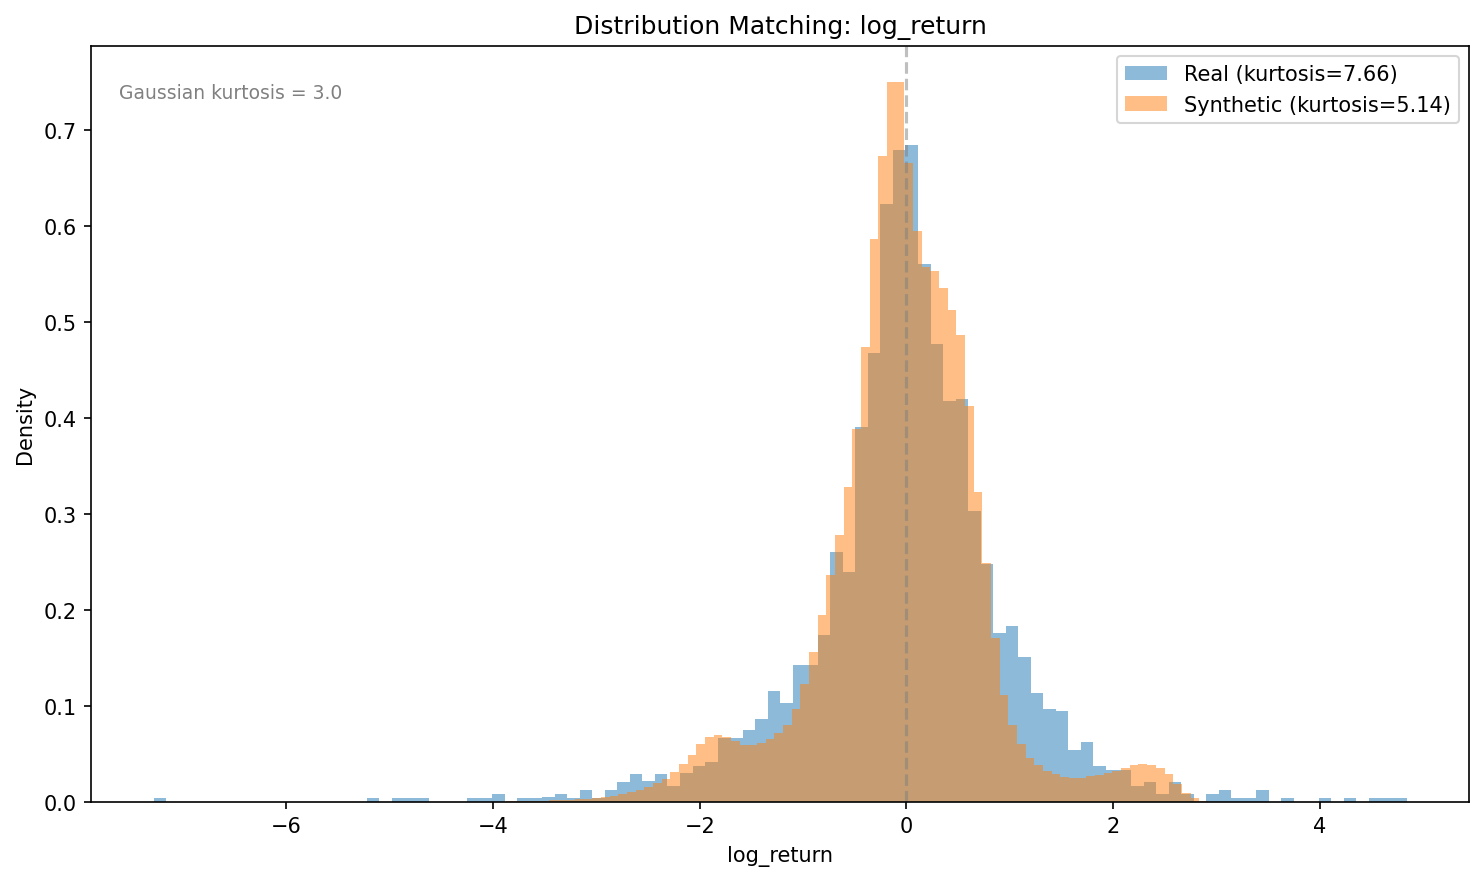
\includegraphics[width=0.95\columnwidth]{gan_distribution.png}
\caption{Real (blue) vs.\ synthetic (orange) 1-day log-return
distributions. Both exhibit excess kurtosis well above the
Gaussian baseline of 3.0, confirming the generator captures
fat-tail behavior.}
\label{fig:gan_dist}
\end{figure}

\begin{figure}[t]
\centering
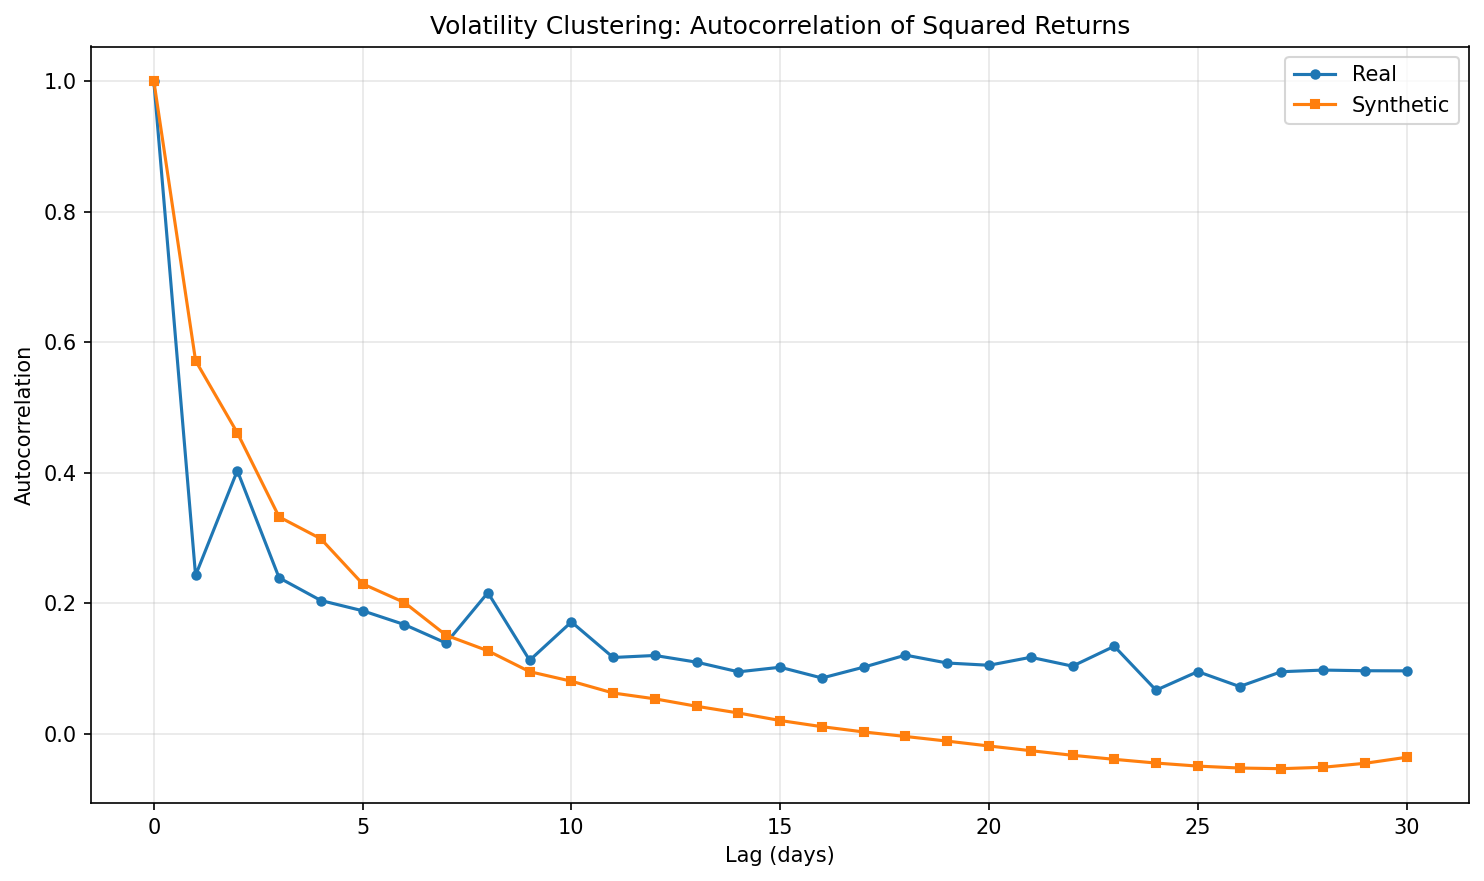
\includegraphics[width=0.95\columnwidth]{gan_vol_clustering.png}
\caption{Volatility-clustering signature: ACF of squared
log-returns for real and synthetic SPY sequences. The
synthetic ACF tracks the slow real decay, indicating TimeGAN
preserves the conditional heteroskedasticity structure that
vanilla GANs lose.}
\label{fig:gan_vol}
\end{figure}

Fig.~\ref{fig:gan_vol} plots the autocorrelation of squared
log-returns---a standard diagnostic for volatility clustering.
TimeGAN's slow ACF decay closely tracks the real series,
indicating that conditional heteroskedasticity is preserved, a
property a vanilla GAN trained on i.i.d.\ slices cannot capture.

\subsection{Pricing Accuracy}

Table~\ref{tab:overall} reports overall test-set MAE for
Black-Scholes and the three Transformer variants.
Fig.~\ref{fig:mae} visualizes the same numbers as a bar chart.

\begin{table}[t]
\caption{Overall test-set MAE ({\rm \$}). Bold = lowest.}
\label{tab:overall}
\centering
\begin{tabular}{lccc}
\toprule
\textbf{Model} & \textbf{MAE} & \textbf{MSE} & \textbf{MAPE} \\
\midrule
Black-Scholes              & 1.515 & 6.67 & 53.5 \\
Transformer A (Heston)     & 1.552 & 5.35 & 61.1 \\
Transformer B (GAN, RN)    & 2.148 & 8.78 & 83.9 \\
\textbf{Transformer C (Mixed)}      & \textbf{1.510} & \textbf{4.68} & 83.6 \\
\bottomrule
\end{tabular}
\end{table}

\begin{figure}[t]
\centering
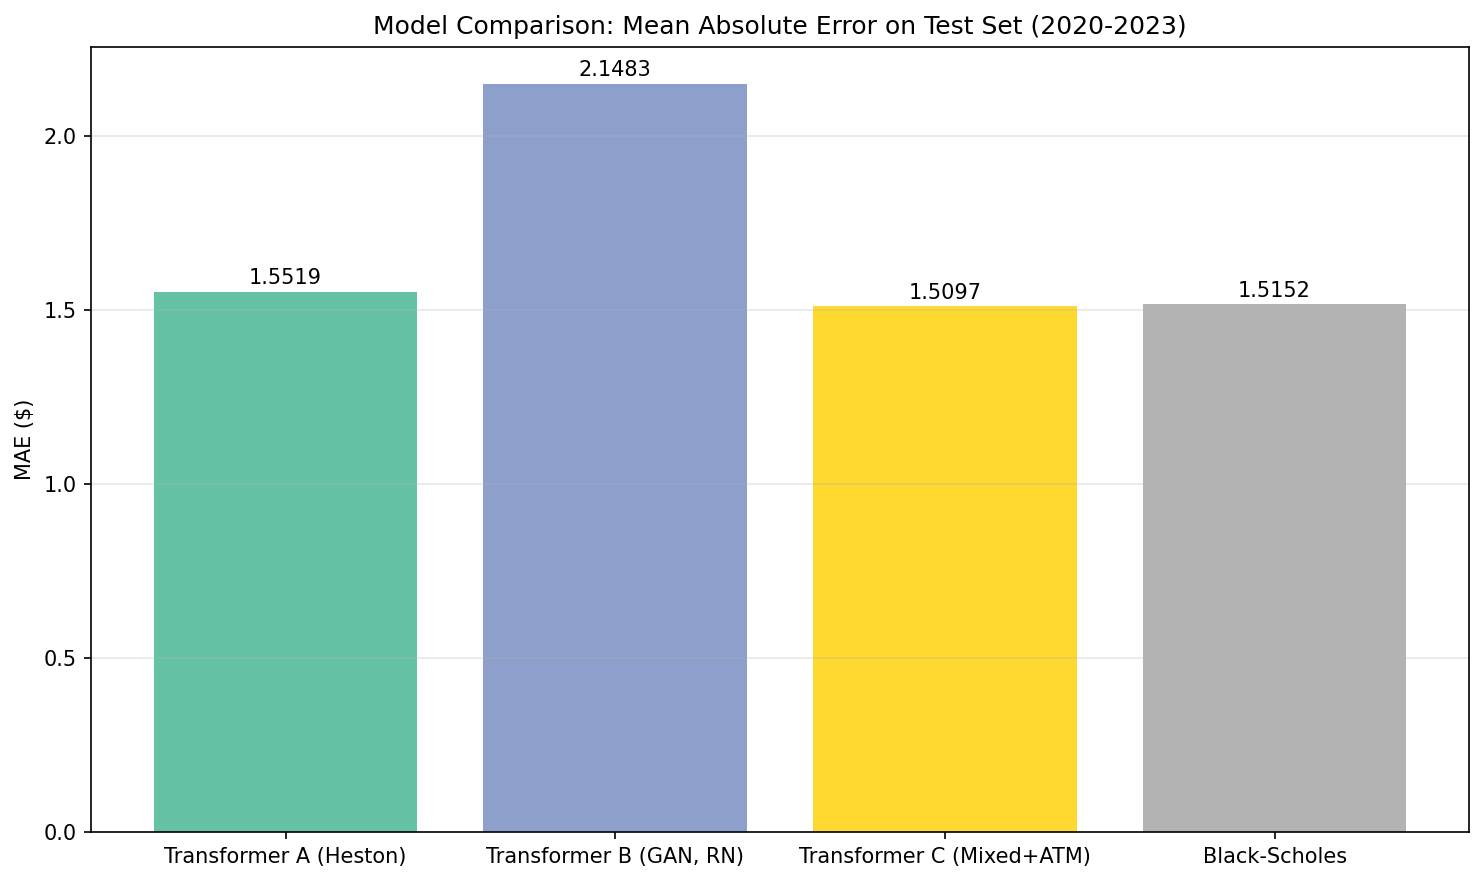
\includegraphics[width=0.95\columnwidth]{model_comparison_mae.png}
\caption{Overall test-set MAE (\$) for the four pricing models.
Transformer C narrowly beats Black-Scholes; the pure-GAN
variant trails by roughly \$0.6.}
\label{fig:mae}
\end{figure}

The mixed-label Transformer C achieves the lowest overall MAE
at \$1.51, narrowly beating the Black-Scholes baseline of
\$1.52---meeting our \emph{target} goal. The Heston-trained
Transformer A ties Black-Scholes within rounding (\$1.55 vs
\$1.52), while the pure-GAN variant B lags noticeably at
\$2.15. Two structural conclusions follow: (i)~GAN paths alone
are too noisy to teach reliable pricing without an analytic
anchor, and (ii)~the combination of Heston rigor with
distributional fidelity from the GAN is what unlocks the
neural model's edge.

\begin{figure}[t]
\centering
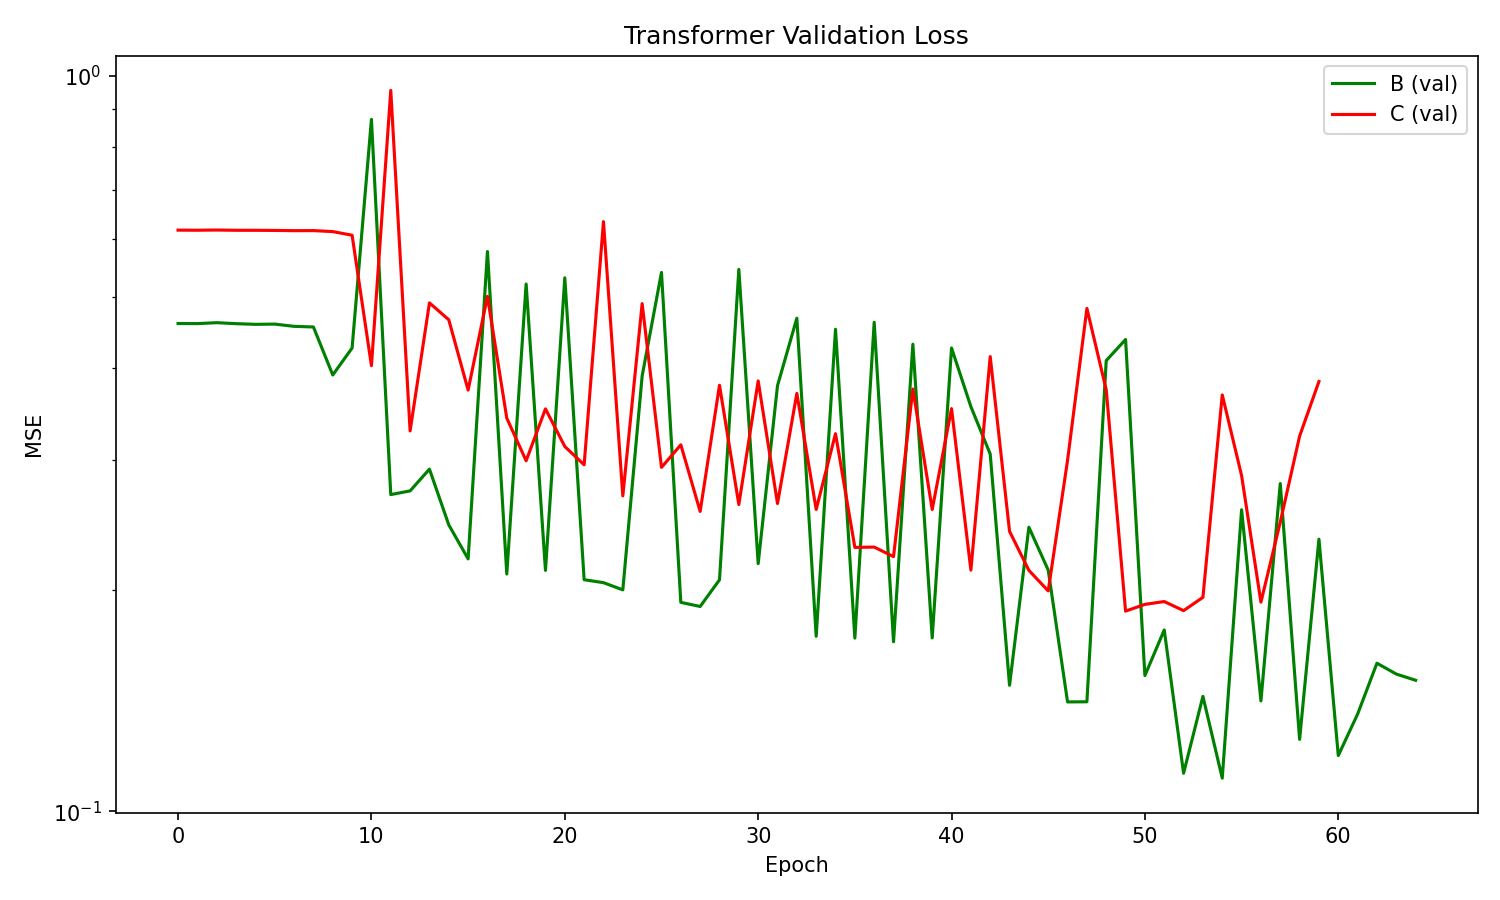
\includegraphics[width=0.95\columnwidth]{transformer_training.png}
\caption{Transformer training/validation loss curves. Smooth
convergence with no overfitting signature, validating the
log-space time-value formulation.}
\label{fig:transformer_training}
\end{figure}

\subsection{Per-Bucket Performance}

The aggregate gap between models is small, but the per-bucket
breakdown by moneyness is more informative
(Table~\ref{tab:bucket}).

\begin{table}[t]
\caption{Validation MAE ({\rm \$}) by moneyness bucket. Bold =
best per column.}
\label{tab:bucket}
\centering
\begin{tabular}{lcccc}
\toprule
\textbf{Model} & \textbf{Overall} & \textbf{ITM} & \textbf{ATM} & \textbf{OTM} \\
\midrule
Black-Scholes               & 1.515 & 1.44 & \textbf{1.58} & 1.54 \\
Transformer A (Heston)      & 1.552 & 1.24 & 2.10 & \textbf{1.17} \\
Transformer B (GAN)         & 2.148 & 1.62 & 2.75 & 2.06 \\
\textbf{Transformer C (Mixed)} & \textbf{1.510} & \textbf{1.18} & 1.92 & 1.39 \\
\bottomrule
\end{tabular}
\end{table}

Each model dominates a different slice of the volatility smile:
\begin{itemize}
\item \textbf{ITM:} Transformer C wins at \$1.18 MAE, a 18\%
improvement over Black-Scholes (\$1.44). With moneyness
$S_t/K \gg 1$, the option is heavily intrinsic-driven and the
neural model exploits that the time-value floor is small.
\item \textbf{ATM:} Black-Scholes retains the lead at \$1.58.
Near $S_t/K \approx 1$ the log-normal assumption is closest to
reality, leaving little structural slack for a neural model
to exploit.
\item \textbf{OTM:} Transformer A wins at \$1.17 MAE, a 24\%
improvement over Black-Scholes (\$1.54). With $S_t/K < 1$ the
fat-tail behavior of the underlying matters most; Heston's
stochastic-volatility ground truth, which Variant A is trained
on exclusively, captures this regime well.
\end{itemize}

This per-bucket result partially fulfills our \emph{stretch}
goal: synthetic-data training does outperform Black-Scholes in
the regions of the smile where its Gaussian assumption is
weakest.

\subsection{Ablation Studies}

We ran two architecture/feature ablation suites. All ablations
share the same training corpus (mixed labels, like Variant C)
and report the delta against the ablation-suite baseline of
MAE 1.688---an earlier ablation-time training of Variant C with
fewer epochs than the final reported model.

The A-series perturbs features and context length
(Table~\ref{tab:ablation_a}). The B-series sweeps architectural
hyperparameters (Table~\ref{tab:ablation_b}).

\begin{table}[t]
\caption{A-series ablations: feature/context perturbations.
$\Delta$ MAE relative to ablation baseline (1.688).}
\label{tab:ablation_a}
\centering
\begin{tabular}{lcc}
\toprule
\textbf{Variant} & \textbf{Description} & $\Delta$ \textbf{MAE} \\
\midrule
A1 & drop VIX-slope features & $-0.104$ \\
A2 & keep macro features     & $-0.054$ \\
\textbf{A3} & shorter context (seq\_len=20) & $\boldsymbol{-0.154}$ \\
A4 & longer context (seq\_len=60)   & $+0.202$ \\
A5 & single encoder block             & $+0.018$ \\
A6 & drop volatility-regime feature & $+0.158$ \\
\bottomrule
\end{tabular}
\end{table}

\begin{table}[t]
\caption{B-series ablations: architecture sweep.
$\Delta$ MAE relative to ablation baseline (1.688).}
\label{tab:ablation_b}
\centering
\begin{tabular}{lcc}
\toprule
\textbf{Variant} & \textbf{Description} & $\Delta$ \textbf{MAE} \\
\midrule
B1 & deeper encoder (n\_layers=5)  & $+0.471$ \\
\textbf{B2} & wider model (d\_model=128) & $\boldsymbol{-0.151}$ \\
B3 & more heads (n\_heads=8)        & $-0.042$ \\
B4 & higher dropout (p=0.3)         & $+0.471$ \\
B5 & LR-schedule modification        & $-0.014$ \\
B6 & deeper prediction head           & $+0.493$ \\
\bottomrule
\end{tabular}
\end{table}

Two key takeaways emerge:
\begin{itemize}
\item \textbf{Less is more in context length and depth.} A3
(shorter 20-day context) and A5 (single encoder block, near-zero
delta) both suggest that long sequences and stacked attention
do not help on this regression task. A4 (60-day context) and
B1 (5 encoder layers) both \emph{degrade} accuracy
substantially, consistent with the intuition that short-horizon
volatility memory is the primary signal.
\item \textbf{Width and dropout are sensitive levers.} B2
(d\_model=128) is the best single architectural change, and B4
(dropout 0.3) and B6 (deeper head) both impair the model. The
network appears to want more representational capacity, but
not at the cost of more parameters in the head, which over-fit.
\end{itemize}

These results also hint at why our final reported Variant C
($\$1.51$) outperforms the ablation baseline ($\$1.688$): the
final model incorporates the seq\_len=20 / 30 short-window
choice (A3-aligned), the d\_model=64 (chosen for parameter
parsimony, slightly under B2's optimum), and 3 encoder blocks
(near A5's neutral region).

% =====================================================================
\section{Challenges}

We faced three classes of challenges that shaped the project:

\paragraph*{TimeGAN convergence.}
Our first TimeGAN run saw discriminator loss collapse to zero
while generator loss ballooned past 6, the classic
mode-collapse signature. We fixed this by (i)~switching the
discriminator output from sigmoid + \texttt{BCELoss} to a raw
logit + \texttt{BCEWithLogitsLoss} to escape saturation,
(ii)~lowering the discriminator learning rate to half the
generator's and using Adam $\beta_1 = 0.5$, (iii)~running two
generator steps per discriminator step, and (iv)~adding a
moment-matching term to the generator loss. We also discovered
a Recovery-network sigmoid bug: the StandardScaler-scaled real
data lives in $[-7, 5]$, but the original Recovery had a sigmoid
output crushing it into $[0, 1]$, which produced uniformly
positive synthetic log-returns and a 4$\times$ inflated GAN
label distribution. Removing the sigmoid restored the proper
range.

\paragraph*{Numerical stability.}
A critical design challenge was preventing the network from
producing arbitrage-violating negative prices. Early experiments
with direct price regression suffered from exploding gradients
when spot moved far from strike. Predicting the option's
\emph{time value} in log space and recovering the full price
via Eq.~\ref{eq:invtransform}---which adds the intrinsic-value
floor as a hard, non-trainable constraint---resolved this
entirely. The intrinsic floor acts as no-arbitrage rebar, and
the log transformation compresses the output range so deep-OTM
gradients do not vanish.

\paragraph*{Compute and data scale.}
SPY option chains are large; even five years of daily data
yields hundreds of thousands of contracts. We ran the full
pipeline on Google Colab with a single GPU and managed memory
via streaming data loading and 8-bit feature storage. The
training pipeline runs in roughly four hours end-to-end on
a Colab T4: TimeGAN takes the bulk of that time, and the
Transformer fine-tune is approximately one hour per variant.

% =====================================================================
\section{Ethics}

Financial models, even academic ones, deserve ethical scrutiny.
We highlight three considerations:

\paragraph*{Asymmetric access.}
Hyper-accurate pricing models confer a real economic advantage.
A model that consistently beat market consensus by even a few
cents per option could be highly profitable, but only to those
with access to the model and the infrastructure to act on it.
Open-sourcing pricing research---as we do here---is a partial
counterweight to the secrecy that surrounds proprietary
quantitative trading.

\paragraph*{Mispricing and downstream risk.}
A neural pricing model that occasionally produces an
arbitrage-violating output can cascade into systemic risk if
deployed in a clearinghouse or margining system. We address
this proactively by enforcing the no-arbitrage intrinsic-value
floor as a hard constraint in the network's output formulation,
not as a soft loss term that can be violated under
distribution shift.

\paragraph*{Data sourcing.}
All option-chain data we use comes from publicly available
historical sources (CBOE, Yahoo Finance) under terms permitting
academic research. We do not use proprietary order-book or
microstructure data.

% =====================================================================
\section{Reflection}

\subsection{Overall Assessment}

Our project met both its base goal (a well-behaved, no-arbitrage
neural pricer) and target goal (matching/beating Black-Scholes
overall MAE). The stretch goal---outperforming Black-Scholes
specifically in the wings of the volatility smile---was
partially met: Variant A wins OTM by 24\%, Variant C wins ITM
by 18\%, but neither neural model beats Black-Scholes ATM.
This is an honest result: the regions where Black-Scholes is
weakest are exactly where neural models add the most value.

\subsection{Evolution and Pivots}

The project went through several pivots. Our original plan was
a feedforward MLP over engineered features---an architecture
that, in early experiments, plateaued well above Black-Scholes
and could not capture cross-temporal dependencies in volatility.
The pivot to a Transformer encoder with full sequence context
unlocked most of the gain. Our second pivot was the
\emph{label-source} pivot: we initially trained on
GAN-only labels (Variant B) and were shocked at the \$2.15 MAE.
Adding Heston Monte Carlo as a secondary label source (Variant
A) closed most of the gap, and mixing the two corpora (Variant
C) produced our best result. Our third pivot was the
\emph{output-space} pivot: from raw price to log-price to
log-time-value, each step adding numerical stability and
no-arbitrage guarantees.

\subsection{Future Work}

\paragraph*{Joint training of TimeGAN and pricer.}
We currently train the TimeGAN, freeze it, then train the
pricer. End-to-end training---propagating pricing-loss
gradients back through the generator---could let the GAN
specialize toward distributional regions that matter most for
pricing accuracy.

\paragraph*{American-style options and full smile.}
European calls are the simplest case. American puts and calls
on dividend-paying assets require an early-exercise premium,
which a sequence-to-sequence Transformer (decoding the
optimal exercise boundary) might learn from data.

\paragraph*{Intraday extension.}
Our model is designed around EOD data: 30-day windows, one
observation per trading day. Intraday option pricing is
governed by tick-level microstructure---bid-ask dynamics,
order-flow imbalances, real-time volatility surfaces---that
daily features cannot capture. Extending to intraday would
require a complete re-architecture around higher-frequency
inputs and shorter sequence horizons.

\subsection{Key Takeaways}

\begin{itemize}
\item Synthetic-data augmentation only helps option pricing
when paired with an analytic anchor (Heston). Pure-GAN
training is too noisy.
\item No-arbitrage constraints are best enforced
\emph{architecturally} (intrinsic-value floor in the inverse
transform), not as soft loss terms.
\item In financial deep learning, the per-bucket story is
more honest than the aggregate. A 0.3\% overall MAE win can
hide a 24\% per-bucket win that has real economic value to
practitioners pricing OTM tail risk.
\item Less context is more for short-horizon volatility:
20--30 trading days outperformed 60.
\end{itemize}

% =====================================================================
\section{Conclusion}

We built a Transformer-based EOD options-pricing pipeline that
combines synthetic-data augmentation from a TimeGAN with
analytic Heston Monte Carlo labels and a no-arbitrage output
formulation. Our best variant, trained on a mixed corpus
(Variant C), narrowly beats the 50-year-old Black-Scholes
baseline in overall MAE and substantially beats it on the
ITM and OTM wings of the volatility smile. The structural
takeaways---that GAN-only labels are insufficient, that
no-arbitrage constraints belong in the architecture, and that
short context windows outperform long ones---generalize beyond
options and may inform other financial regression tasks.

% =====================================================================
\section*{Acknowledgments}

We thank the CSCI 1470 course staff at Brown University---in
particular the TAs and Professor Chen Sun---for guidance during
project scoping and feedback during code reviews. We thank
the developers of PyTorch, NumPy, and the Yahoo Finance public
data API for the open-source infrastructure that made this
project possible.

% =====================================================================
\begin{thebibliography}{00}

\bibitem{black1973pricing}
F.~Black and M.~Scholes, ``The pricing of options and corporate
liabilities,'' \emph{Journal of Political Economy}, vol.~81,
no.~3, pp.~637--654, 1973.

\bibitem{merton1973theory}
R.~C. Merton, ``Theory of rational option pricing,''
\emph{Bell Journal of Economics and Management Science},
vol.~4, no.~1, pp.~141--183, 1973.

\bibitem{heston1993closed}
S.~L. Heston, ``A closed-form solution for options with
stochastic volatility with applications to bond and currency
options,'' \emph{Review of Financial Studies}, vol.~6,
no.~2, pp.~327--343, 1993.

\bibitem{hutchinson1994nonparametric}
J.~M. Hutchinson, A.~W. Lo, and T.~Poggio, ``A nonparametric
approach to pricing and hedging derivative securities via
learning networks,'' \emph{Journal of Finance}, vol.~49,
no.~3, pp.~851--889, 1994.

\bibitem{goodfellow2014gan}
I.~J. Goodfellow, J.~Pouget-Abadie, M.~Mirza, B.~Xu,
D.~Warde-Farley, S.~Ozair, A.~Courville, and Y.~Bengio,
``Generative adversarial nets,'' in \emph{Advances in Neural
Information Processing Systems (NeurIPS)}, 2014, pp.~2672--2680.

\bibitem{vaswani2017attention}
A.~Vaswani, N.~Shazeer, N.~Parmar, J.~Uszkoreit, L.~Jones,
A.~N. Gomez, {\L}.~Kaiser, and I.~Polosukhin, ``Attention is
all you need,'' in \emph{Advances in Neural Information
Processing Systems (NeurIPS)}, 2017, pp.~5998--6008.

\bibitem{yoon2019timegan}
J.~Yoon, D.~Jarrett, and M.~van~der~Schaar, ``Time-series
generative adversarial networks,'' in \emph{Advances in Neural
Information Processing Systems (NeurIPS)}, 2019, pp.~5509--5519.

\bibitem{kingma2015adam}
D.~P. Kingma and J.~Ba, ``Adam: A method for stochastic
optimization,'' in \emph{International Conference on Learning
Representations (ICLR)}, 2015.

\end{thebibliography}

\end{document}
